\documentclass[a4paper,11pt]{article}

\usepackage[latin1]{inputenc}
\usepackage[T1]{fontenc}
\usepackage{bbm} %math chars
\usepackage{amsmath}
\usepackage{indentfirst}
\usepackage{fullpage} %minimizes the default margins
\usepackage{url}
\usepackage{graphicx}
\usepackage[center,footnotesize]{caption} %options des legendes des graphes
\usepackage[section]{placeins} %place les figures d'une section avant le debut de la suivante
\usepackage{subfig} %a) b) c)

\title{Exercises - Week 9}
\date{}
\author{Genomics and bioinformatics}

\begin{document}
\maketitle

\section{The Fitch's algorithm}

\noindent Applying the Fitch's algorithm to each column separately, we find:
\begin{figure}[h!]
\centering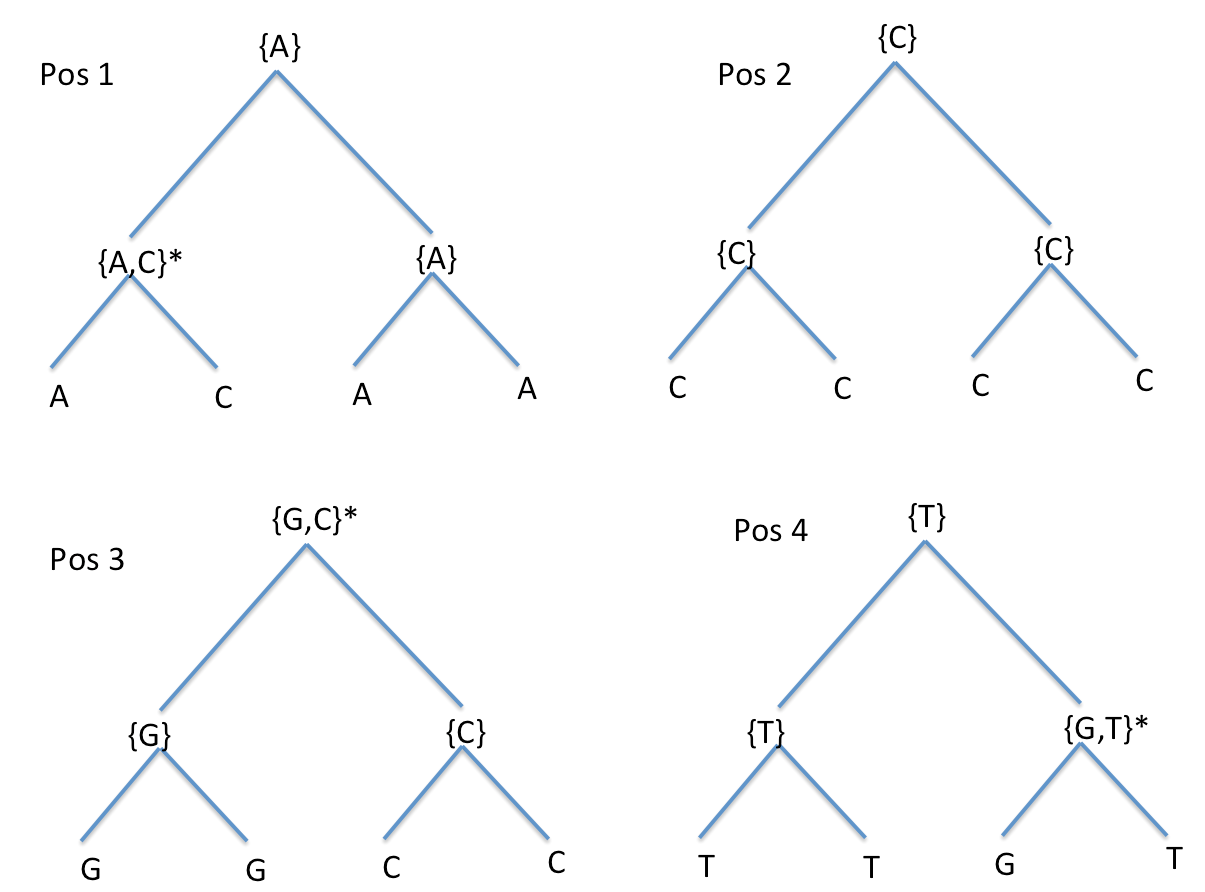
\includegraphics[width=14cm]{Fig1.png}
\end{figure}

\noindent There are two assignments of the states to the internal nodes, with a parsimony length $L(T)=3$.
\begin{figure}[h!]
\centering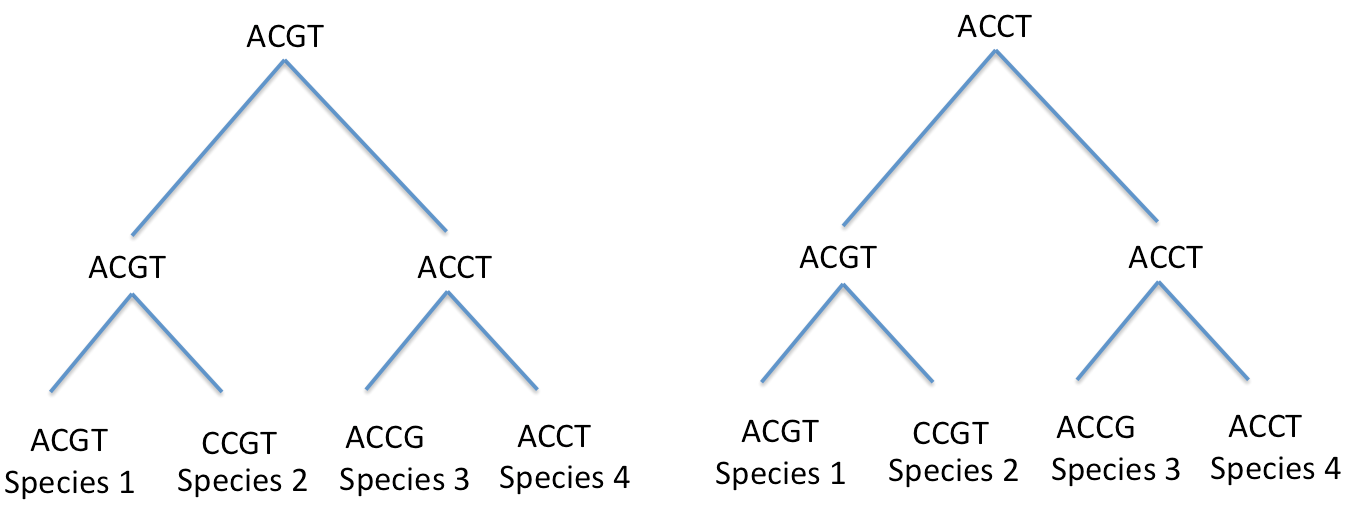
\includegraphics[width=14cm]{Fig2.png}
\end{figure}

\section{The Sankoff's algorithm}

\noindent Applying the Sankoff's algorithm to the first column of the MSA, we find:
\begin{figure}[h!]
\centering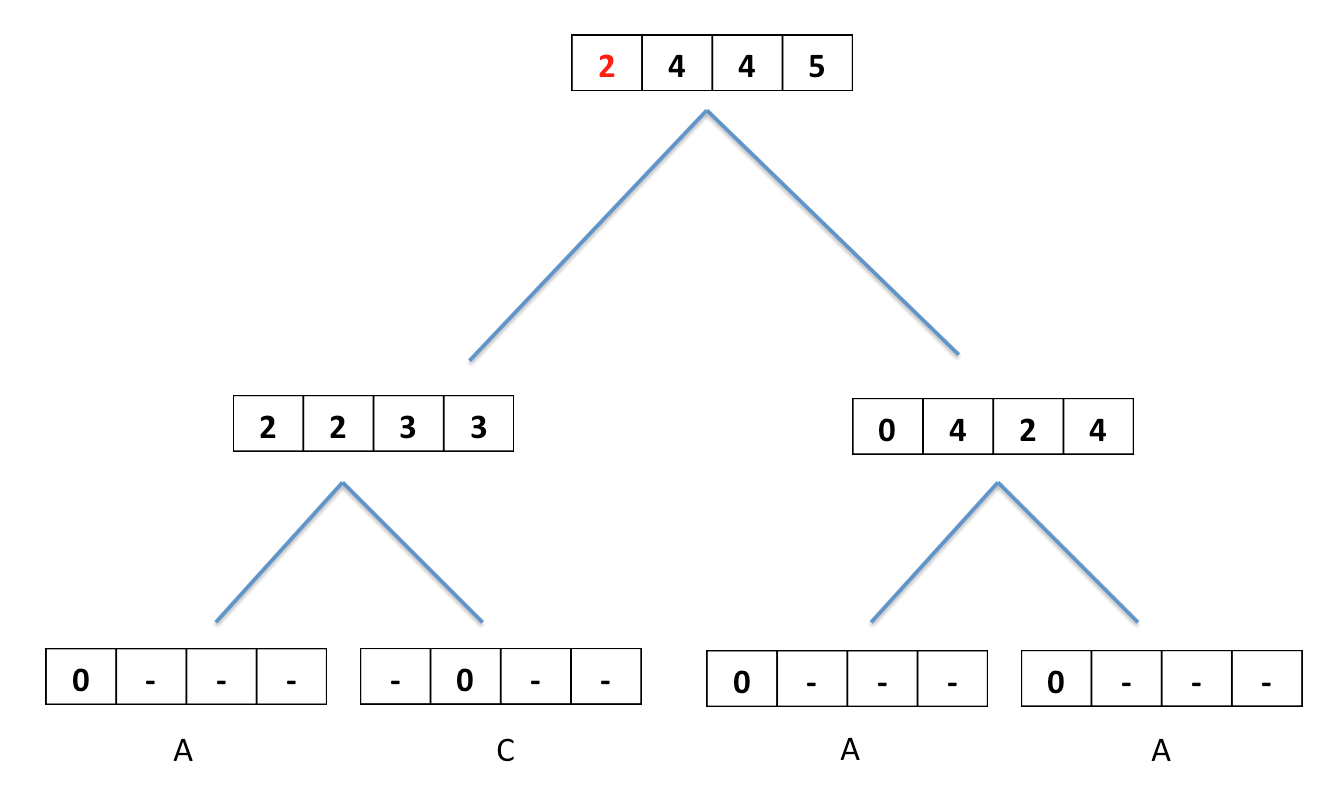
\includegraphics[width=12cm]{Fig3.png}
\end{figure}

\noindent The score of the tree is equal to the minimum of the root values, which is 2. This means that given the first column of the MSA and the substitution matrix $M$, one needs at least a penalty of 2 with respect to mutations to explain this tree.

\section{The UPGMA algorithm}

\begin{figure}[h!]
\centering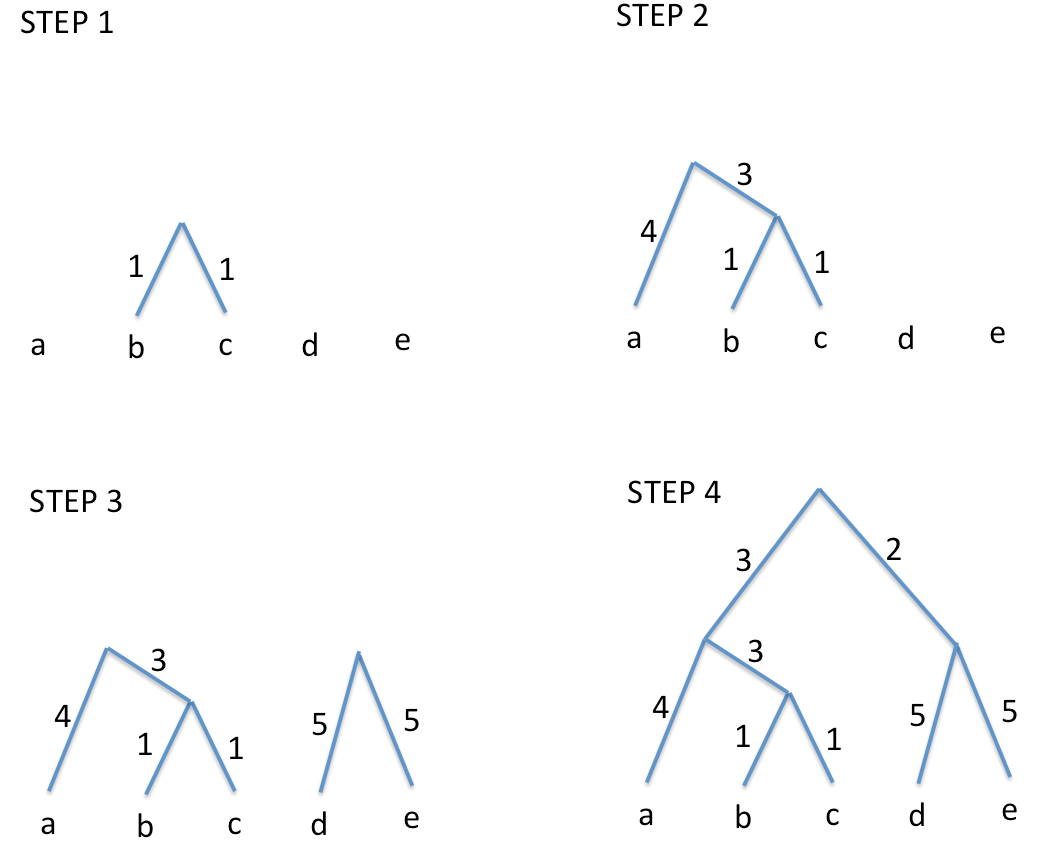
\includegraphics[width=13cm]{Fig4.png}
\end{figure}


\end{document}











